\documentclass[]{article}

%opening
\title{Exercises Set 6}
\author{Paul Dubois}

\usepackage{amsmath}
\usepackage{amsfonts}
\usepackage{amsthm}
\usepackage{amssymb}
\usepackage{mathrsfs}
\usepackage{stmaryrd}
\usepackage{graphicx}

\newcommand{\Q}{\mathbb{Q}}
\newcommand{\N}{\mathbb{N}}
\newcommand{\Z}{\mathbb{Z}}
\newcommand{\R}{\mathbb{R}}
\newcommand{\Primes}{\mathbb{P}}
\newcommand{\st}{\text{ s.t. }}
\newcommand{\txtand}{\text{ and }}
\newcommand{\txtor}{\text{ or }}
\newcommand{\lxor}{\veebar}


\begin{document}
	
	\maketitle
	
	\begin{abstract}
		Only the questions with a * are compulsory (but do all of them!).
	\end{abstract}	
	
	\section{Lagrangian multiplier technique}
	\begin{center}
		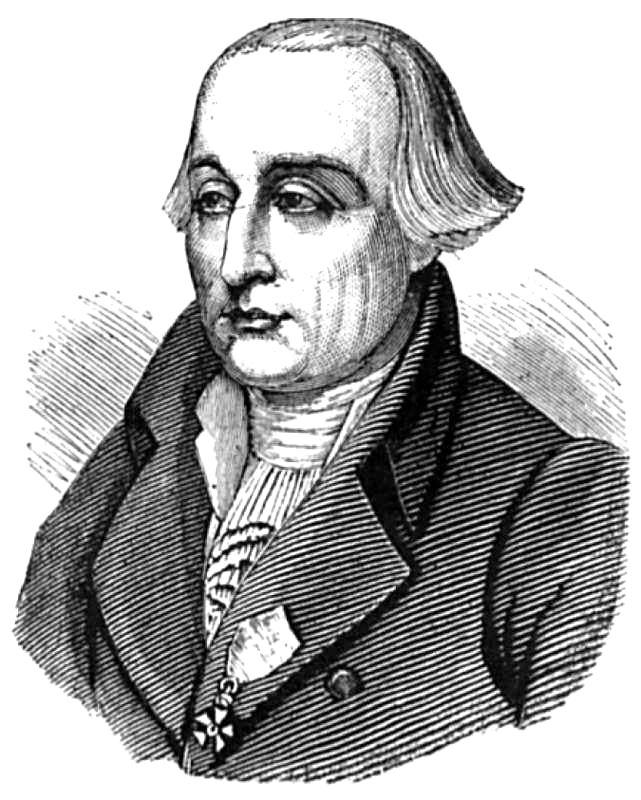
\includegraphics[height=4cm]{Lagrange}
	\end{center}

	\subsection{Unconstrained optimization}
	Let $f(x,y) = 2x^2-3x + 4y^2 + 4y +20$.\\
	Find $(x^*,y^*) \in \R^2$ such that $f$ reaches its minimum (i.e. $f(x^*,y^*) \leq f(x,y) \quad \forall (x,y) \in \R^2$).
	
	\subsection{Constrained optimization}
	Let $f(x,y) = 2x^2-3x + 4y^2 + 4y +20$.\\
	Suppose further that we want $3x + 5y = 2$.\\
	Find $(x^*,y^*) \in \R^2$ such that $3x^* + 5y^* = 2$ and $f$ reaches its minimum (i.e. $f(x^*,y^*) \leq f(x,y) \quad \forall (x,y) \in \R^2,\ 3x + 5y = 2$).
	
	\subsection{Lagrange multiplier}
	Let $f(x,y) = 2x^2-3x + 4y^2 + 4y +20$.\\
	Suppose further that we want $3x + 5y = 2$.\\
	Let $\mathcal{L}(x,y,\lambda) = f(x,y) - \lambda (3x + 5y -2)$.\\
	Find the point where $\nabla f = 0$
	
	
	
\end{document}
